\chapter{Geheugencel}
\label{cell}
De meeste geheugens bestaan uit een verzameling individuele cellen die op een manier informatie bevatten.
In dit hoofdstuk wordt dieper ingegaan op de manier waarop een RRAM geheugencel informatie bevat.

\section{Memristor}
Het essentiële element van de RRAM geheugencel in dit werk is de zogenaamde memristor.
De memristor wordt ook wel gezien als de 4\textsuperscript{e} passieve component, naast de weerstand, spoel en condensator.

\subsection{Theoretisch principe}
In 1971 publiceerde Leon Chua, een onderzoeker in o.a. niet-lineaire circuittheorie, een artikel waarin hij opmerkte dat er voor de 4 fundamentele circuitvariabelen (de spanning v, stroom i, lading q en flux $\phi$\footnote{$\phi(t) =  \int^{t}_{-\infty} v(\tau) \, d\tau $, voor een ideale inductantie is dit hetzelfde als magnetische flux}) van 6 mogelijke onderlinge relaties er slechts 5 gekend waren: $q(t) =  \int^{t}_{-\infty} i(\tau) \, d\tau $, $\phi(t) =  \int^{t}_{-\infty} v(\tau) \, d\tau $, $v(t)=R*i(t)$, $q(t)=C*v(t)$ en $\phi(t) = L*i(t)$ volgen uit de wetten van Maxwell en uit de definities van de weerstand, spoel en condensator, maar er ontbrak een relatie tussen $\phi$ en q\cite{Chu71}. Hij suggereerde dat er een 4e nog niet ontdekte passieve 2-pool moest bestaan die dit verband herbergde. Hij stelde dat $M(q)= \frac{d\phi(q)}{dq}$ met M de \emph{memristance}.
Hieruit volgt dat voor dit element $v(t)=M(q(t)) i(t)$. Indien er een lineair verband bestaat tussen $\phi$ en q, gedraagt dit element zich als een gewone weerstand. Enkel wanneer er een niet-lineair verband bestaat, beginnen er zich interessante karakteristieken voor te doen. Zo gedraagt het element zich ogenblikkelijk als een weerstand, maar gaat deze weerstandswaarde variëren in de tijd aan de hand van de stroom die er doorgelopen heeft.
Gebaseerd op deze conclusie doopte hij deze component de memristor, een contractie van memory en resistor.
Chua beëindigde zijn artikel met te erkennen dat er op dat moment nog geen fysische memristor was ontdekt, maar dat dit in de toekomst wel kon gebeuren, al dan niet zelfs per ongeluk. Hij gaf zelfs aan dat er misschien al in die tijd materialen met memristorkarakteristieken gebruikt werden, maar dat men hier over keek. Hij zou gelijk krijgen.

\subsection{Fysische memristors}
Er werd reeds langer (zelfs al sinds de jaren 60) opgemerkt dat sommige metaaloxides, die normaal gezien als elektrisch isolator functioneren, een plotse overgang kunnen ervaren naar een veel geleidendere staat (zie figuur \ref{fig:i-v}). Dit gebeurt veelal in een configuratie waarbij het oxide wordt geplaatst tussen 2 metalen (MIM configuratie)\cite{Won12} (zie ook figuur \ref{fig:mim}).

\begin{figure}
  \centering
  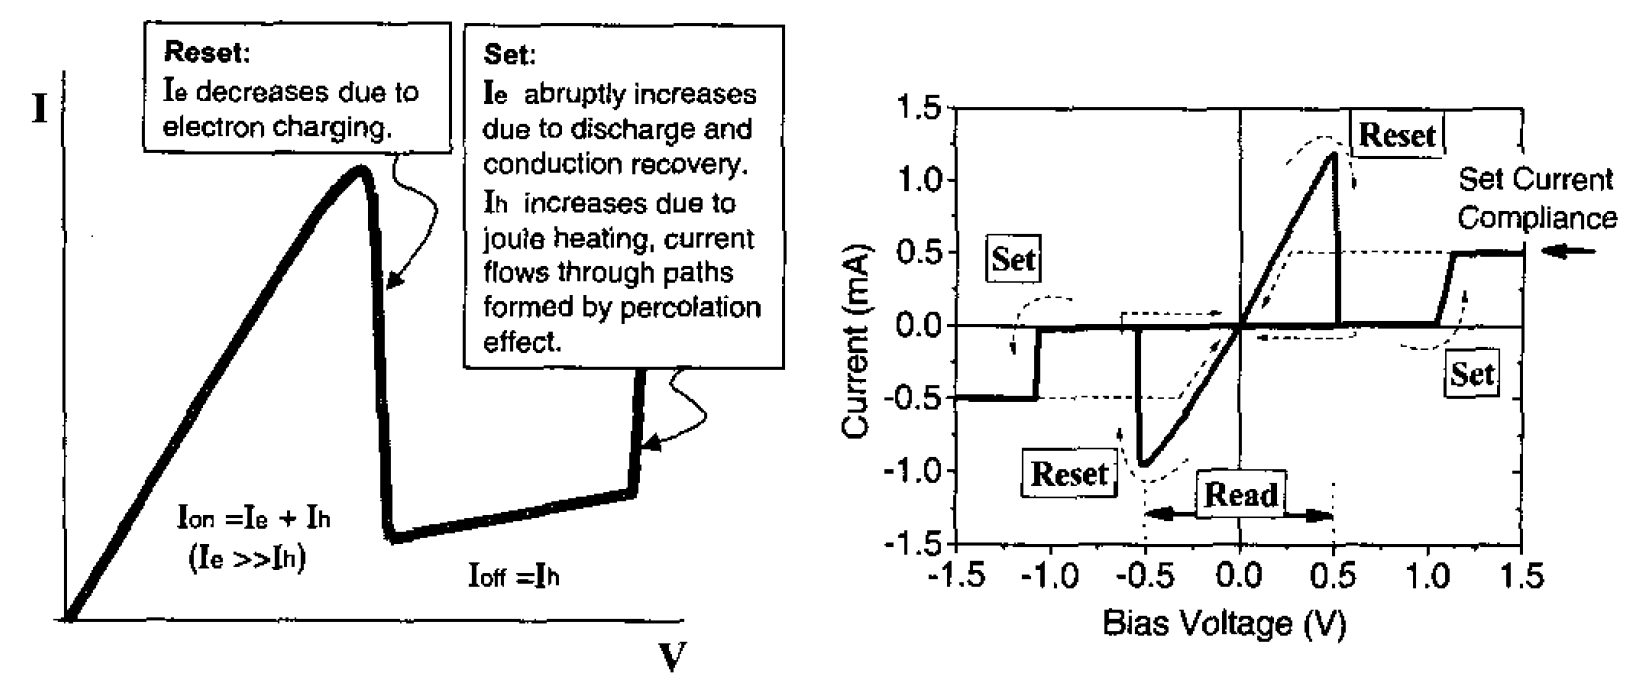
\includegraphics[scale=0.25]{../fig/hfdstk-cel-I-V.png}
  \caption[Resistieve schakeling]{Abrupte overgang van hoge weerstand naar lage weerstand voor NiO, reproduced from\cite{Bae04}}
  \label{fig:i-v}
\end{figure}

\begin{figure}
  \centering
  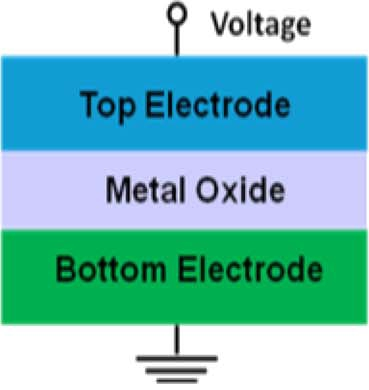
\includegraphics[scale=0.4]{../fig/hfdstk-cel-MIM.png}
  \caption[MIM structuur]{Metal-Insulator-Metal structuur, reproduced from\cite{Won12}}
  \label{fig:mim}
\end{figure}

In 2008 publiceerde een onderzoeksgroep van Hewlett-Packard een artikel waarin ze opmerkten dat het gedrag van hun Pt-TiO\textsubscript{2}-Pt stalen een merkwaardige gelijkenis vertoonde met Chua's memristor.\cite{Str08} Uit de modellering van hun stalen argumenteerden ze dat dit een ideale memristor zou zijn en dat het effect meer uitgesproken is bij kleine afmetingen: het titaniumoxide bestaat uit 2 delen: zuiver TiO\textsubscript{2}, een halfgeleider met hoge weerstand, en TiO\textsubscript{2-x} met zuurstofafwezigheid (oxygen vacancies) met een veel lagere weerstand. Door een elektrisch veld aan te leggen worden zuurstofatomen weg of in het rooster getrokken en verandert de verhouding TiO\textsubscript{2} en TiO\textsubscript{2-x} en dus ook de netto weerstand (zie figuur \ref{fig:HP-model}).

\begin{figure}
  \centering
  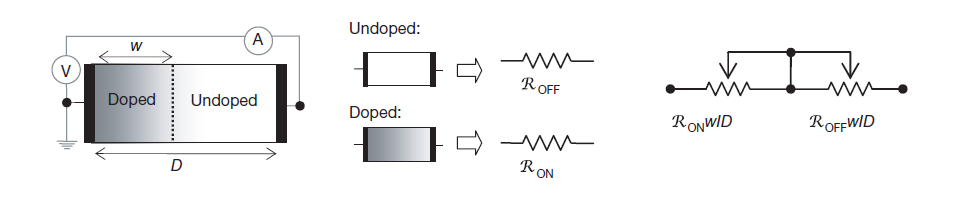
\includegraphics[scale=0.5]{../fig/hfdstk-cel-HP-model.png}
  \caption[Model van het Pt-TiO\textsubscript{2}-Pt staal]{Model van het Pt-TiO\textsubscript{2}-Pt staal, reproduced from\cite{Str08}}
  \label{fig:HP-model}
\end{figure}

Voor deze opstelling geldt dan dat $M(q)=R\textsubscript{off}(1-\frac{\mu\textsubscript{v}R\textsubscript{on}}{D^2}q(t))$ met D de dikte van de titaniumoxidefilm, $\mu\textsubscript{v}$ de mobiliteit van de zuurstofionen en $R\textsubscript{on} \leq M \leq R\textsubscript{off}$. Het dymamisch gedrag van de ogenblikkelijke weerstandswaarde is dus afhankelijk van het verloop van de stroom in de tijd en dit des te meer in het nanometerdomein.

Naast titaniumoxide zijn er nog andere materialen die schakelend weerstandsverdrag vertonen zoals nikkeloxide\cite{Bae04}, hafniumoxide\cite{Che11}, aluminiumoxide\cite{Kim06},... Niet altijd kunnen de resultaten gemodelleerd worden volgens de originele memristortheorie, maar desalnietemin zullen deze materiaalconfiguraties bruikbaar zijn in toepassingen.
Bij al deze MIM-configuraties blijft het mechanisme wel hetzelfde: na fabricatie is het oxidekristal intrinsiek zuiver, maar onder druk van een voldoende groot elektrisch veld zullen de zuurstofatomen losgerukt worden uit het rooster naar de anode. Het gebrek aan zuurstofatomen zorgt voor conductieve filamenten. Het element bereikt dan een laagresistieve staat (LRS).
Deze zachte doorslag van het zuivere oxide wordt \emph{forming} genoemd. Het proces is tot zekere hoogte omkeerbaar (\emph{reset}), maar er zullen altijd meer defecten in het kristal zijn dan voor de forming. Dit betekent dus ook dat nadat de memristor één keer een forming- en resetproces is ondergaan en zich terug in een hoogresistieve staat (HRS) bevindt, er hierna een minder groot elektrisch veld nodig is om terug tot een LRS te komen. Dit proces heet \emph{setting}. Deze drie processen zijn geïllustreerd op figuur \ref{fig:forming-reset-set}.

\begin{figure}
  \centering
  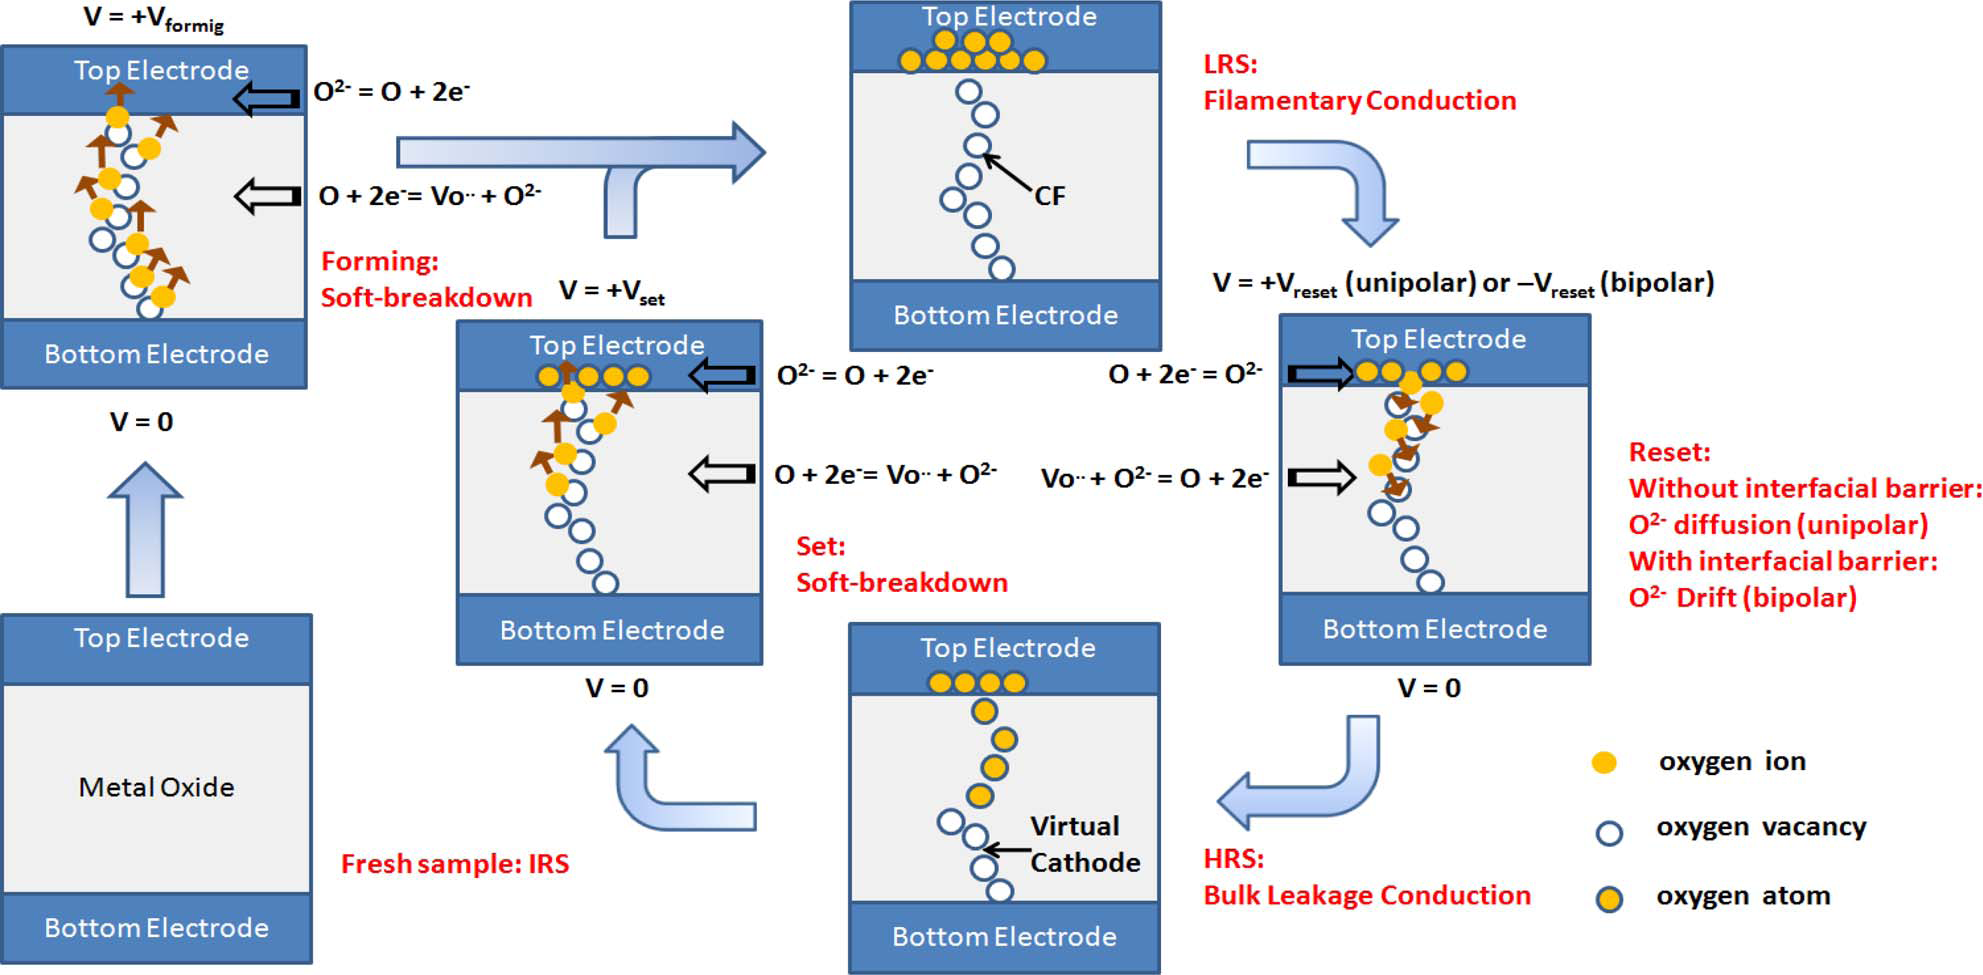
\includegraphics[scale=0.22]{../fig/hfdstk-cel-forming-reset-set.png}
  \caption[Forming,resetting en setting van een memristor]{Illustratie van forming,resetting en setting, reproduced from\cite{Won12}}
  \label{fig:forming-reset-set}
\end{figure}

De verschillende MIM-structuren hebben ook verschillende eigenschappen. Zo moet er onderscheid gemaakt worden tussen unipolair schakelen en bipolair. Bij bipolair resistief schakelen zal forming/setting optreden wanneer de aangelegde spanning een bepaalde polariteit heeft en resetting bij de omgekeerde polariteit. Bij unipolair schakelen is de amplitude of de duur van de spanning doorslaggevend voor welke van de 3 processen zal optreden, niet de polariteit. 


\section{Memristortoepassingen}
\label{1T1R}

Voor dit werk is het voor de hand liggend dat de memristor gebruikt kan worden als geheugenelement: de MIM-configuraties hebben op z'n minst 2 resistieve toestanden, al zijn er artikels gepubliceerd waarbij de memristor nog meer resistieve toestanden bevat\cite{Liu12}. Als deze multiresistive states onder controle gehouden kunnen worden, kan een nog hogere densiteit aan informatie gerealiseerd worden aangezien elke memristor meer dan 1 bit informatie zou bevatten (multi-level cells).
Deze 2 toestanden kunnen gebruikt worden voor geheugen- en logicatoepassingen\cite{ros12}\cite{raj09}. In geheugentoepassingen kan men onderscheid maken tussen 1T1R-,1R- en 1D1R-configuraties\cite{Den13}. Met een 1R-configuratie kan men de grootste densiteit van geheugen bereiken, alsook een betere schaling, maar deze configuratie heeft te kampen met cellen die maar half geselecteerd worden. Dit kan opgelost worden door een selectie-element aan de configuratie toe te voegen, zoals een diode of een transistor. De 1D1R configuratie kan echter enkel geïmplementeerd worden met unipolaire memristors\cite{Wou09}. Daarom dat er in dit werk voor een 1T1R-configuratie geopteerd werd, de memristor waarop dit werk bebaseerd is, is immers een bipolaire hafniumoxide-memristor (zie figuur \ref{fig:1T1R}).

\begin{figure}
  \centering
  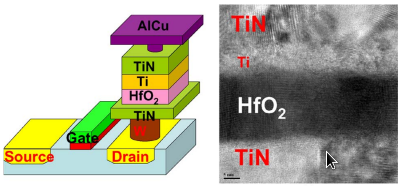
\includegraphics[scale=0.6]{../fig/hfdstk-cel-1T1R.png}
  \caption[Een 1T1R-configuratie]{Een 1T1R-configuratie, reproduced from\cite{Won12}}
  \label{fig:1T1R}
\end{figure}

Naast geheugentoepassingen heeft de memristor ook potentieel in logicatoepassigen, er wordt zelfs gesproken over een volledige vervanger van de transistor\cite{Kue05}.

\subsection{1T1R-cel}
De 1T1R-celarchitectuur is niet alleen van toepassing bij RRAM, ook bij STT-MRAM wordt deze celstructuur gebruikt.

\section{Besluit}
De memristor is een theoretische passieve component die lading en flux met elkaar verbindt. In de praktijk zijn er MIM-configuraties ontdekt die memristorkarakteristieken vertonen. Deze karakteristieken zijn bijzonder interessant voor geheugens: gecombineerd met een transistor vormt de memristor een 1T1R-geheugencel, die geïmplementeerd wordt in de volgende hoofdstukken.
